\documentclass[]{article}
\usepackage{amsmath}
\usepackage{amsthm}
\usepackage{listings}
%\usepackage[margin=1.3cm]{geometry}
\usepackage{graphicx}
\usepackage{hyperref}

\title{Practical Lab Numerical Computing Computational Finance \\Bachelor-Worksheet 4}
\author{Lukas Troska, Ilja Kalmykov}
\date{}
\setlength{\parindent}{0pt}

\begin{document}

\maketitle

The source code can be found at \url{https://github.com/iljaGH/CompFin/}.

\section*{Task 1}
Integrand of 2 dimensional Down-Out call option $S(0)=10,K=10,B=8,T=1,\sigma=0.2,r=0.05$.\\
\begin{figure}[!ht]
\centering
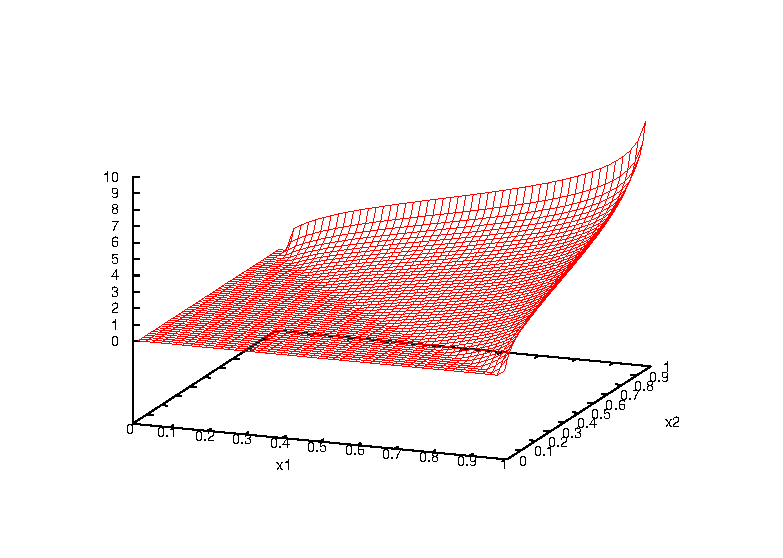
\includegraphics[width=.9\textwidth]{task1.eps}
\caption{Integrand of 2 dimensional Down-Out call option}
\label{fig:Task1}
\end{figure}
\clearpage


\section*{Task 2}
Discrete Down-Out call option with $M=128,S(0)=10,K=10,B=9,T=1,\sigma=0.2,r=0.05$.\\
Below are the convergence plots for Monte Carlo and Quasi-Monte Carlo respectively using the closed-form solution as a reference value. We can see that the Randomwalk path discretization is more suitable for this particular integration problem. The third plot is a pseudo convergence plot for Monte Carlo using a low precision reference value (4 significant figures). The error is very low for a short time, because we "pass" the low precision reference value during the convergence. Then the error stabilizes at the relative error between the low reference value and the actual limit.

\begin{figure}[!ht]
\centering
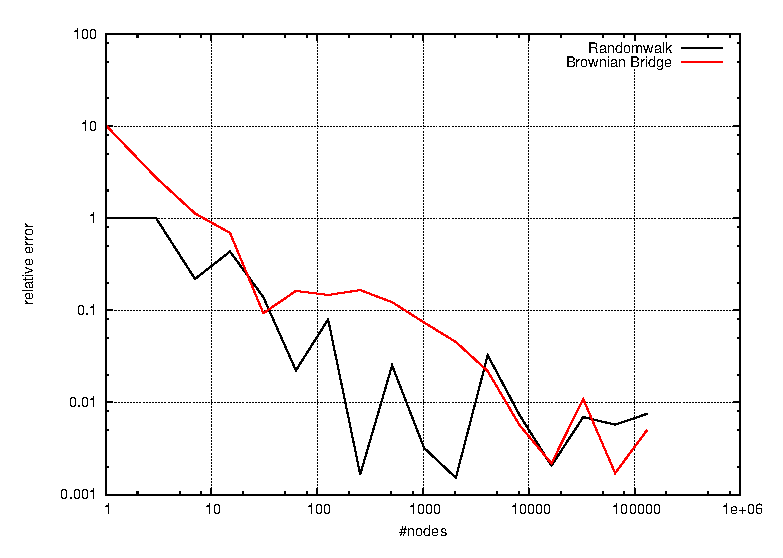
\includegraphics[width=.9\textwidth]{task2_mc_high.eps}
\caption{Convergence plot for Monte Carlo}
\label{fig:Task2a}
\end{figure}

\begin{figure}[!ht]
\centering
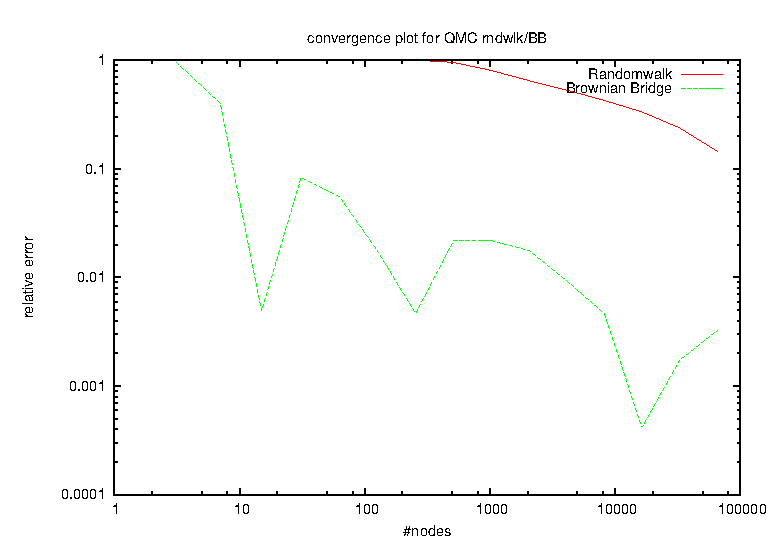
\includegraphics[width=.9\textwidth]{task2_qmc.eps}
\caption{Convergence plot for Quasi-Monte Carlo}
\label{fig:Task2b}
\end{figure}

\begin{figure}[!ht]
\centering
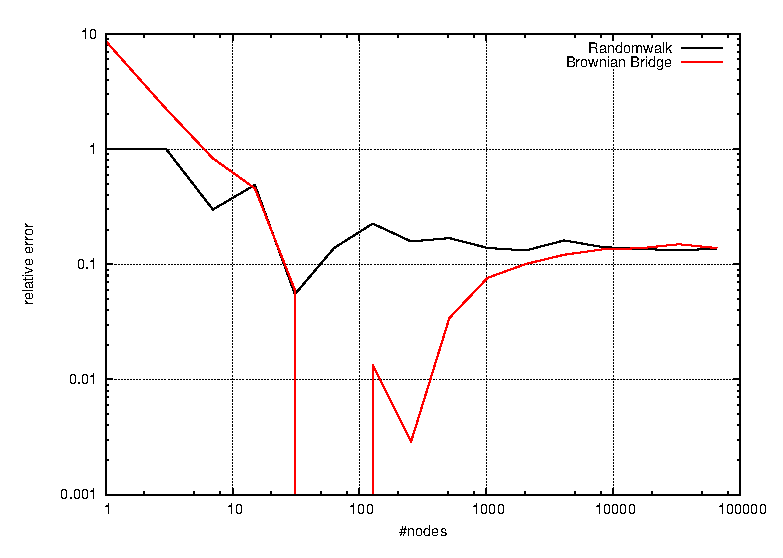
\includegraphics[width=.9\textwidth]{task2_mc_low.eps}
\caption{Convergence plot for Monte Carlo with low precision reference value (4 significant figures)}
\label{fig:Task2c}
\end{figure}
\clearpage

\section*{Task 3}
Fair price of Down-Out call option with  $S(0)=10,K=10,T=1,\sigma=0.2,r=0.05$ for varying $B$ using the Black-Scholes formula.
\begin{figure}[!ht]
\centering
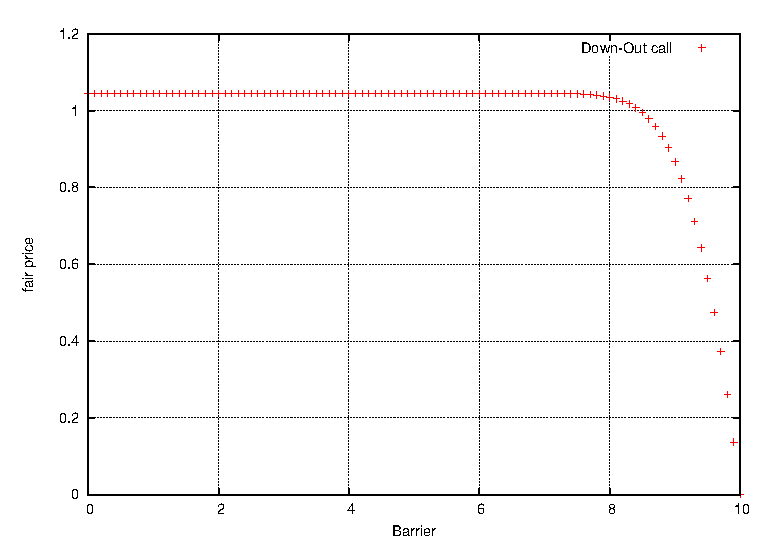
\includegraphics[width=.9\textwidth]{task3.eps}
\caption{Fair price of Down-Out call options, varying barrier}
\label{fig:Task3}
\end{figure}
\clearpage


\section*{Task 4}
Convergence of Down-Out call option with $S(0)=10,K=10,B=9,T=1,\sigma=0.2,r=0.05$, varying $M$, against closed form solution using Monte Carlo.
\begin{figure}[!ht]
\centering
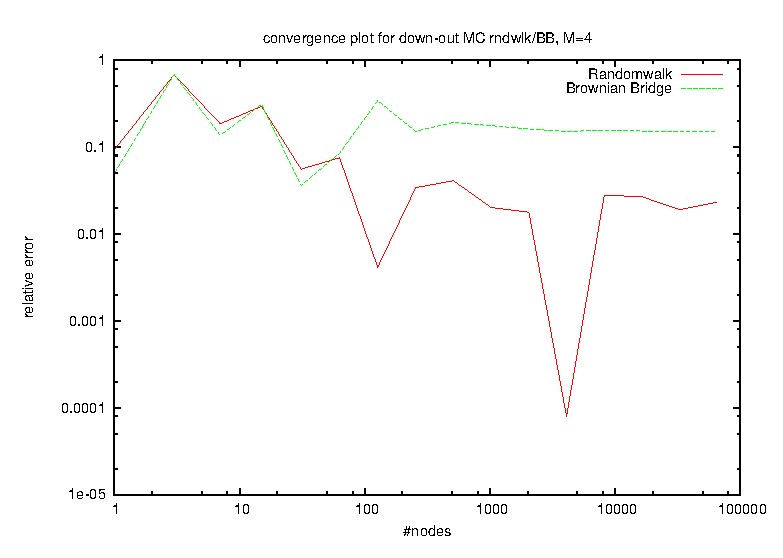
\includegraphics[width=.9\textwidth]{task4_mc_4.eps}
\caption{Convergence plot for $M=4$}
\label{fig:Task4a}
\end{figure}

\begin{figure}[!ht]
\centering
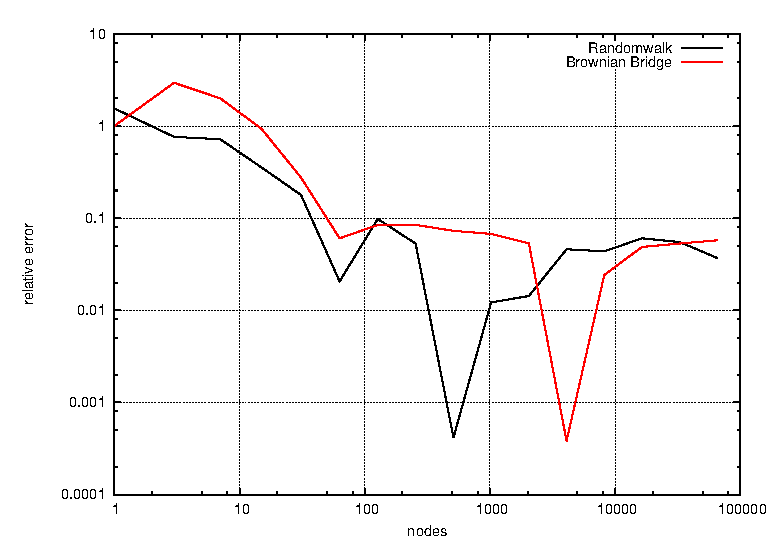
\includegraphics[width=.9\textwidth]{task4_mc_64.eps}
\caption{Convergence plot for $M=64$}
\label{fig:Task4b}
\end{figure}

\begin{figure}[!ht]
\centering
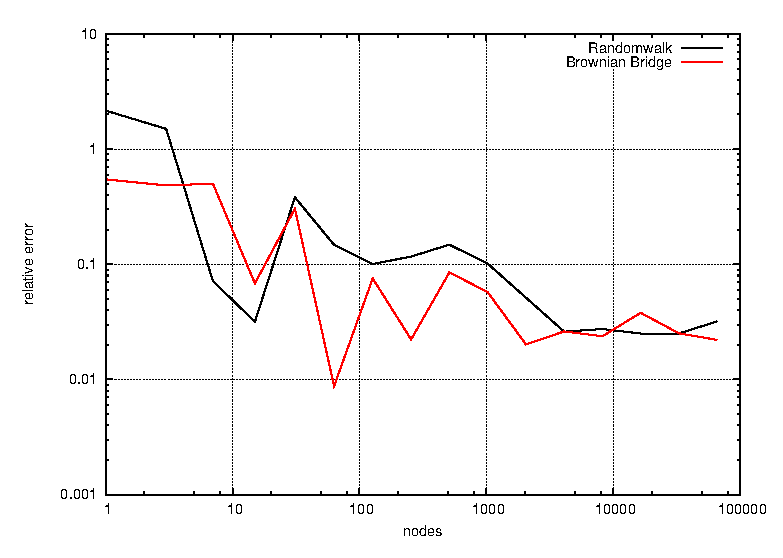
\includegraphics[width=.9\textwidth]{task4_mc_256.eps}
\caption{Convergence plot for $M=256$}
\label{fig:Task4c}
\end{figure}

\begin{figure}[!ht]
\centering
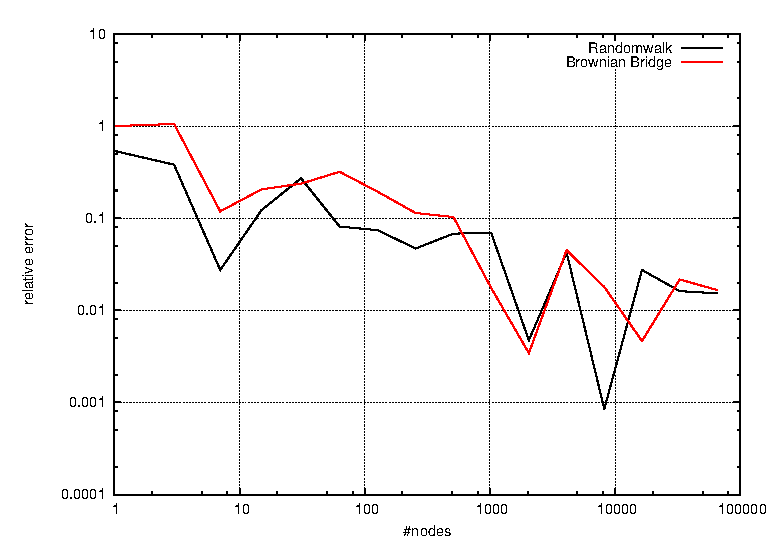
\includegraphics[width=.9\textwidth]{task4_mc_1024.eps}
\caption{Convergence plot for $M=1024$}
\label{fig:Task4d}
\end{figure}

\begin{figure}[!ht]
\centering
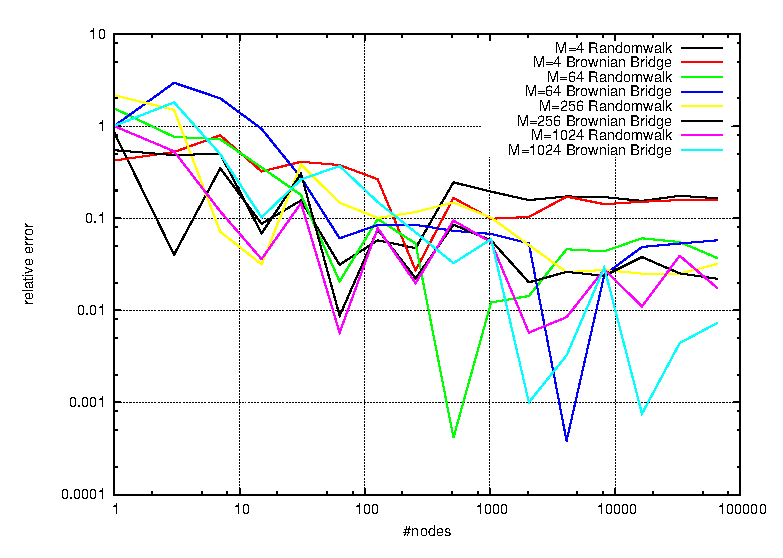
\includegraphics[width=.9\textwidth]{task4_mc.eps}
\caption{Comparison of all plots above}
\label{fig:Task4e}
\end{figure}
\clearpage

\section*{Task 5}
Integrand of a discrete time Lookback option with $M=2,S(0)=10,K=10,\\T=1,\sigma=0.2,r=0.05$.
\begin{figure}[!ht]
\centering
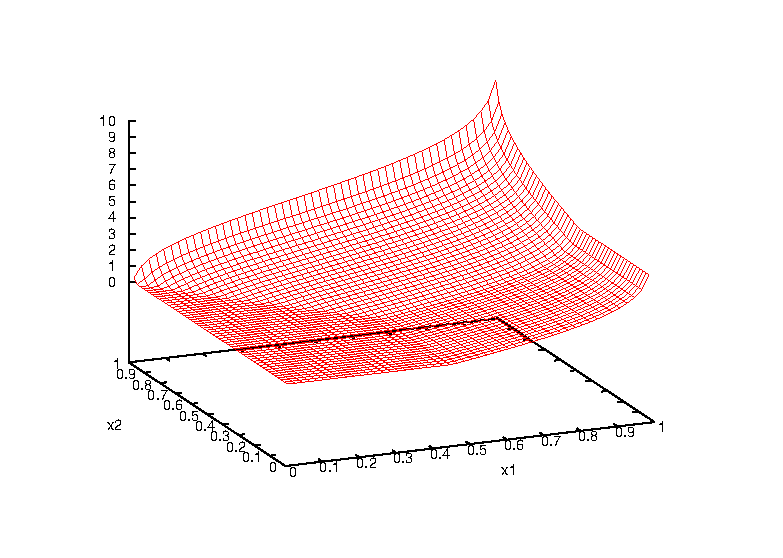
\includegraphics[width=.9\textwidth]{task5.eps}
\caption{Integrand for discrete time Lookback option}
\label{fig:Task5}
\end{figure}
\clearpage

\section*{Task 6}
Convergence of a discrete time Lookback option with $M=128,S(0)=10,K=10,T=1,\sigma=0.2,r=0.05$ using Monte Carlo and Quasi-Monte Carlo with Brownian Bridge discretization against closed-form solution.
\begin{figure}[!ht]
\centering
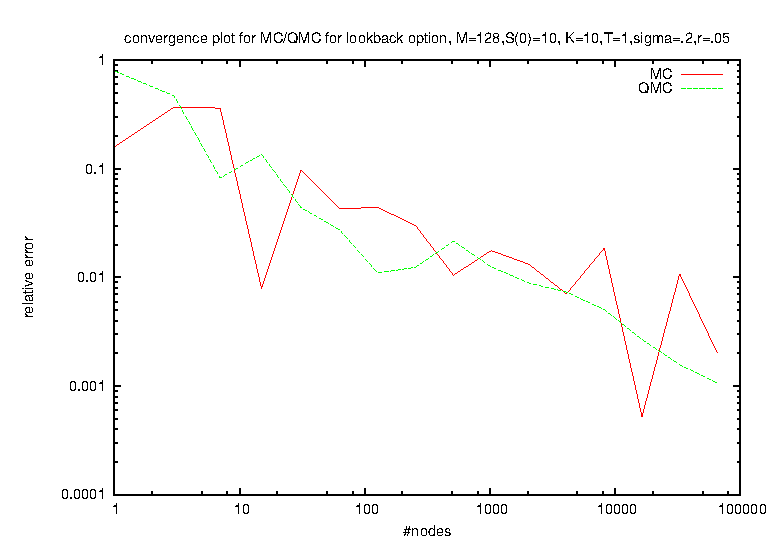
\includegraphics[width=.9\textwidth]{task6.eps}
\caption{Convergence plot for a discrete time Lookback option}
\label{fig:Task6}
\end{figure}

\section*{Task 7}
Implementation of implied volatility. See task7.cpp for code.

\section*{Task 8}
Implementation of bisection method. See task8.cpp for code.
\clearpage

\section*{Task 9}
The following is a plot of the implied volatility of a Lufthansa call option, with $T=0.1$. At the time, Lufthansa stock was worth $19.93$, and the options were valued:\\

\centering
\begin{tabular}[ht]{c|c}
K & V\\
\hline
19.5&0.97\\
19.75&0.79\\
20&0.65€\\
20.25&0.54€\\
20.5&0.44€\\
20.75&0.36€\\
21&0.3€\\
\end{tabular}

\begin{figure}[!ht]
\centering
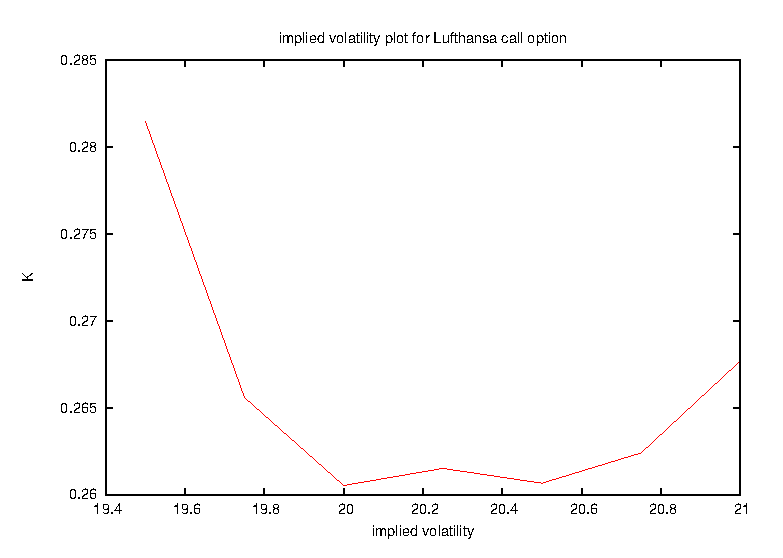
\includegraphics[width=.9\textwidth]{task9.eps}
\caption{Volatility smile, Lufthansa call option}
\label{fig:Task9}
\end{figure}

\end{document}
